\documentclass{article}

\usepackage{fancyhdr,ifthen,calc}

\newif\ifpdf
\ifx\pdfoutput\undefined
\pdffalse % we are not running PDFLaTeX
\else
\pdfoutput=1 % we are running PDFLaTeX
\pdftrue
\fi

\ifpdf
\usepackage[pdftex]{graphicx}
\else
\usepackage{graphicx}
\fi

%%%%%%%%%%%%%%%%%%%%%%%%%%%%%%%%%%%%%%%%%%%%%%%%%%%%%%%%%%%%%%%%%%%%%%%%%
% MANPAGE like description setting for options, use as 
% \begin{Lentry} \item[text] text  \end{Lentry}

\newcommand{\entrylabel}[1]{\mbox{\textsf{#1}}\hfil}
\newenvironment{entry}
  {\begin{list}{}
    {\renewcommand{\makelabel}{\entrylabel}
      \setlength{\labelwidth}{90pt}
      \setlength{\leftmargin}{\labelwidth+\labelsep}
    }
  }
  {\end{list}}

\newlength{\Mylen}
\newcommand{\Lentrylabel}[1]{%
  \settowidth{\Mylen}{\textsf{#1}}%
  \ifthenelse{\lengthtest{\Mylen > \labelwidth}}%
    {\parbox[b]{\labelwidth} %  term > labelwidth
      {\makebox[0pt][l]{\textsf{#1}}\\}} %
    {\textsf{#1}} %

  \hfil\relax}
\newenvironment{Lentry}
  {\renewcommand{\entrylabel}{\Lentrylabel}
   \begin{entry}}
  {\end{entry}}
%%%%%%

\begin{document}

\title{PUGH}
\author{Gabrielle Allen}
\date{2001}
\maketitle

\abstract{The default unigrid driver for Cactus for both multiprocessor and single process runs, handling grid variables and communications.}

\section{Description}

PUGH can create, handle and communicate grid scalars, arrays and functions
in 1, 2 or 3-dimensions.

\section{Compilation}

PUGH can be compiled with or without MPI. Compiling without MPI results
in an executable which can only be used on a single processor, compiling 
with MPI leads to an executable which can be used with either single or
multiple processors.
(Section~\ref{pugh_understanding} describes how you can tell if your
executable has been compiled with or without MPI).

For configuring with MPI, see the Cactus User's Guide.

\section{Grid Size}

The number of grid points used for a simulation can be set in PUGH either
globally (that is, the total number of points across all processors), or 
locally (that is, the number of points on each processor). 

To set the global size of a 2D grid to be $40\times 40$ use

{\tt
\begin{verbatim}
driver::global_nx = 40
driver::global_ny = 40
\end{verbatim}
}

To set the local size of a 2D grid to be $40\times 20$ on each processor, use

{\tt
\begin{verbatim}
pugh::local_nx = 40
pugh::local_ny = 20
\end{verbatim}
}



\section{Periodic Boundary Conditions}

PUGH can implement periodic boundary conditions during the synchronization 
of grid functions. Although this may a first seem a little confusing, and 
unlike the usual use of boundary conditions which are directly called from 
evolution routines, it is the most efficient and natural place for periodic
boundary conditions.

PUGH applied periodic conditions by simply communicating the appropriate 
ghostzones between "end" processors. For example, for a 1D domain with two
ghostzones, split across two processors, Figure~\ref{pugh::fig1} shows the implementation of periodic boundary conditions.

\begin{figure}[ht]
\begin{center}
\ifpdf
\else
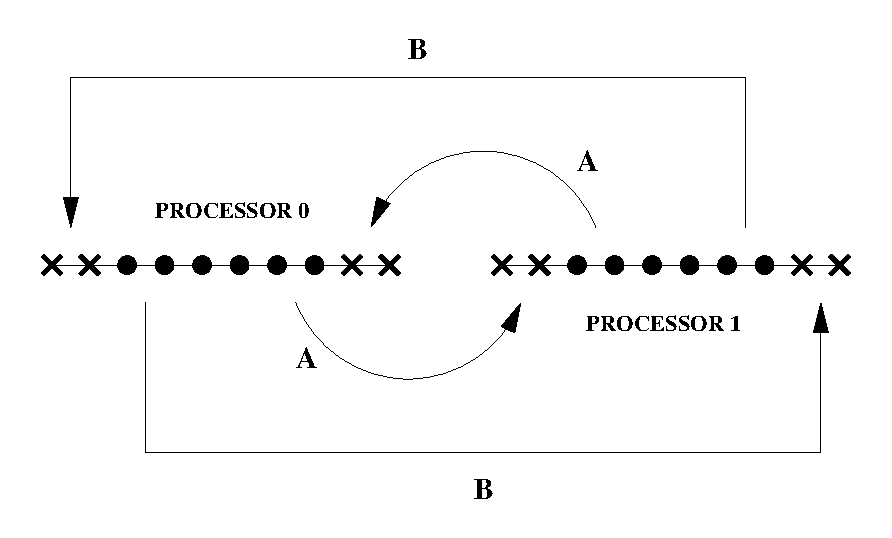
\includegraphics[angle=0,width=8cm]{periodic.eps}
\fi
\end{center}
\caption[]{Implementation of periodic boundary conditions for a 1D domain, with two ghostzones, split across two processors. The lines labelled {\bf A} show the {\it standard} communications during synchronisation, the lines labelled 
{\bf B} show the additional communications for periodic boundary conditions.} 
\label{pugh::fig1}
\end{figure}

Periodic boundary conditions are applied to all grid functions, by default
they are applied in all directions, although this behaviour can be customised
to switch them off in given directions.

By default, no periodic boundary conditions are applied. To apply periodic boundary conditions in all directions, set

{\tt
\begin{verbatim}
driver::periodic = "yes"
\end{verbatim}
}

To apply periodic boundary conditions in just the x- and y- directions or 
a 3 dimension domain, use

{\tt
\begin{verbatim}
driver::periodic = "yes"
driver::periodic_z = "no"
\end{verbatim}
}

\section{Processor Decomposition}

\section{Load Balancing}

By default PUGH will distribute the computational grid evenly across
all processors. This may not be efficient if there is a different
computational load on different processors, or for example for a simulation
distributed across different processor speeds. 

The computational grid can be manually distributed using the parameters
{\tt partition[\_1d\_x|\_2d\_x|\_2d\_y|\_3d\_x|\_3d\_y|\_3d\_z]}. To manual specify the 
load distribution, set {\tt pugh::partition = ``manual''} and then, 
depending on the grid dimension, set the remaining parameters 
to distribute the load in each direction. Note that for this you need
to know apriori the processor decomposition. 

The decomposition is easiest to explain with an example,
to distribute a grid with $30 \times 30$ points across
4 processors (decomposed as $2 \times 2$) as:

\begin{tabular}{cc}
$20\times 15$ & $10 \times 15$ \\
$20\times 15$ & $10 \times 15$ 
\end{tabular}

use the parameters

{\tt
\begin{verbatim}
pugh::partition=''manual''
pugh::partition_2d_x=''20:10''
pugh::partition_2d_y=''15:15''
\end{verbatim}
}


Note that an empty string for a direction will apply the automatic distribution.
\section{Understanding PUGH Output}

\label{pugh_understanding}

PUGH reports information about the processor decomposition to standard output 
at the start of a job. This section described how to interpret that output.

\vskip .3cm

\noindent
{\bf Single Processor (no MPI)}

\begin{itemize}

\item{\bf Type of evolution}

If an executable has been compiled for only single processor use
(without MPI), the first thing which PUGH reports is this fact:

{\tt INFO (PUGH): Single processor evolution}

\end{itemize}


\vskip .3cm

\noindent
{\bf Multiple Processor (with MPI)}



\vskip .3cm

\begin{itemize}

\item{\bf Type of evolution}

If an executable has been compiled using MPI, the first thing which 
PUGH reports is this fact, together with the number of processors
being used:

{\tt INFO (PUGH): MPI Evolution on 3 processors}


\item{\bf Maximum load skew} 

The maximum load skew describes the variance in the number of gridpoints on
each processor, and is defined by

$$\mbox{Max Skew} = 100 \;\;\frac{\mbox{Max Points}- \mbox{Min Points}}{\mbox{Average Points}} $$

For most purposes, the maximum skew should ideally be close to zero,
however if your simulation has a different load at different grid
points, or if you are running across processors with different
properties, the optimal skew could be quite different.

By default, PUGH tries to minize the skew in gridpoints, however this may
be overriden by performing the load balancing manually.

\end{itemize}

\section{Useful Parameters}

There are several parameters in PUGH which are useful for debugging and 
optimisation:

\begin{Lentry}

\item[{\tt pugh::enable\_all\_storage}]

	Enables storage for all grid variables (that is, not only 
	those set in a thorns {\tt schedule.ccl} file). Try this parameter
	if you are getting segmentation faults, if enabling all storage
	removes the problem, it most likely means that you are accessing
	a grid variable (probably in a Fortran thorn) for which storage
	has not been set.

\item[{\tt pugh::initialise\_memory}]

	By default, when PUGH allocates storage for a grid variable it
	does not initialise its elements. If you access an
	uninitialised variable on some platforms you will get a
	segmentation fault (and in general you will see erratic
	behaviour). This parameter can be used to initialise all
	elements to zero, if this removes your segmentation fault you
	can then track down the cause of the problem by using the same
	parameter to initialize all elements to NaNs and then track 
	them with the thorn {\tt CactusUtils/NaNChecker}.

   	Note that it isn't recommended to simply use this parameter to 
	initialise all elements to zero, instead we recommend you to 
	set all variables to their correct values before using them.

\item[{\tt pugh::storage\_verbose}]

	This parameter can be set to print out the number of grid variables
	which have storage allocated at each iteration, and the total 
	size of the storage allocated by Cactus. Note that this total
	does not include storage allocated independently in thorns.

\item[{\tt timer\_output}]

	This parameter can be set to provide the time spent communicating
	variables between processors.

\end{Lentry}


% Automatically created from the ccl files by using gmake thorndoc
\include{interface}
\include{param}
\include{schedule}

\end{document}
